\documentclass[UTF8,a4paper,10pt]{ctexart}
\usepackage[left=2.50cm, right=2.50cm, top=2.50cm, bottom=2.50cm]{geometry}
%页边距
\CTEXsetup[format={\Large\bfseries}]{section} %设置章标题居左

%%%%%%%%%%%%%%%%%%%%%%%
% -- text font --
% compile using Xelatex
%%%%%%%%%%%%%%%%%%%%%%%
% -- 中文字体 --
%\setmainfont{Microsoft YaHei}  % 微软雅黑
%\setmainfont{YouYuan}  % 幼圆    
%\setmainfont{NSimSun}  % 新宋体
%\setmainfont{KaiTi}    % 楷体
%\setmainfont{SimSun}   % 宋体
%\setmainfont{SimHei}   % 黑体
% -- 英文字体 --
%\usepackage{times}
%\usepackage{mathpazo}
%\usepackage{fourier}
%\usepackage{charter}

%\usepackage{helvet}

\usepackage{amsmath, amsfonts, amssymb} % math equations, symbols
\usepackage[english]{babel}
\usepackage{color}	% color content
\usepackage{graphicx}	% import figures
\usepackage{url}	% hyperlinks
\usepackage{bm} 	% bold type for equations
\usepackage{multirow}
\usepackage{booktabs}
\usepackage{epstopdf}
\usepackage{epsfig}
\usepackage{algorithm}
\usepackage{algorithmic}
\usepackage{listings}
\usepackage{xcolor}
\usepackage{booktabs}
\usepackage{zhnumber}
\usepackage{longtable}
\usepackage{subfigure}
\usepackage{float}
\usepackage{caption}
\usepackage{subfigure}
\renewcommand\thesection{\zhnum{section}}
\renewcommand \thesubsection {\arabic{section}}
\renewcommand{\algorithmicrequire}{ \textbf{Input:}}
% use Input in the format of Algorithm  
\renewcommand{\algorithmicensure}{ \textbf{Initialize:}}
% use Initialize in the format of Algorithm  
\renewcommand{\algorithmicreturn}{ \textbf{Output:}}
% use Output in the format of Algorithm  
%%%%%%%%%%%%%%%%%%
\usepackage{listings}
\usepackage{color}
\definecolor{dkgreen}{rgb}{0,0.6,0}
\definecolor{gray}{rgb}{0.5,0.5,0.5}
\definecolor{mauve}{rgb}{0.58,0,0.82}
\lstset{frame=tb,
  language=Python,
  aboveskip=3mm,
  belowskip=3mm,
  showstringspaces=false,
  columns=flexible,
  basicstyle={\small\ttfamily},
  numbers=left,%设置行号位置none不显示行号
  %numberstyle=\tiny\courier, %设置行号大小
  numberstyle=\tiny\color{gray},
  keywordstyle=\color{blue},
  commentstyle=\color{dkgreen},
  stringstyle=\color{mauve},
  breaklines=true,
  breakatwhitespace=true,
  escapeinside=``,%逃逸字符(1左面的键),用于显示中文例如在代码中`中文...`
  tabsize=4,
  extendedchars=false %解决代码跨页时,章节标题,页眉等汉字不显示的问题
}

%%%%%%%%%%%%%%%%%%%%%%%%%%%%
\usepackage{fancyhdr} %设置页眉、页脚
\pagestyle{fancy}
\lhead{}
\chead{}
%\rhead{\includegraphics[width=1.2cm]{fig/ZJU_BLUE.eps}}
\lfoot{}
\cfoot{}
\rfoot{}
\fancyfoot[RE,RO]{~\thepage~}

\fancyhead[RE,RO]{计算物理导论 \quad 2022春季学期 \quad 作业4  \quad 何翼成}

%%%%%%%%%%%%%%%%%%%%%%%
%  设置水印
%%%%%%%%%%%%%%%%%%%%%%%
%\usepackage{draftwatermark}         % 所有页加水印
%\usepackage[firstpage]{draftwatermark} % 只有第一页加水印
% \SetWatermarkText{Water-Mark}           % 设置水印内容
% \SetWatermarkText{\includegraphics{fig/ZJDX-WaterMark.eps}}         % 设置水印logo
% \SetWatermarkLightness{0.9}             % 设置水印透明度 0-1
% \SetWatermarkScale{1}                   % 设置水印大小 0-1    

\usepackage{hyperref} %bookmarks
\hypersetup{colorlinks, bookmarks, unicode} %unicode

\title{\textbf{雪崩数值模拟与次数概率分布}}
\author{ 何翼成 \thanks{学号:520072910043; \newline
    邮箱地址:heyicheng@sjtu. edu. cn} }
\date{\today}

\begin{document}
\maketitle

%\begin{abstract}
%这是一篇中文小论文。这个部分用来写摘要。摘要的章标题默认是英文,还没找到改成中文的方法:(
%\end{abstract}

\section{题目分析}
%%%以下为插入图片模板
%\quad \newline
	\begin{figure}[!htbp]
		\centering
		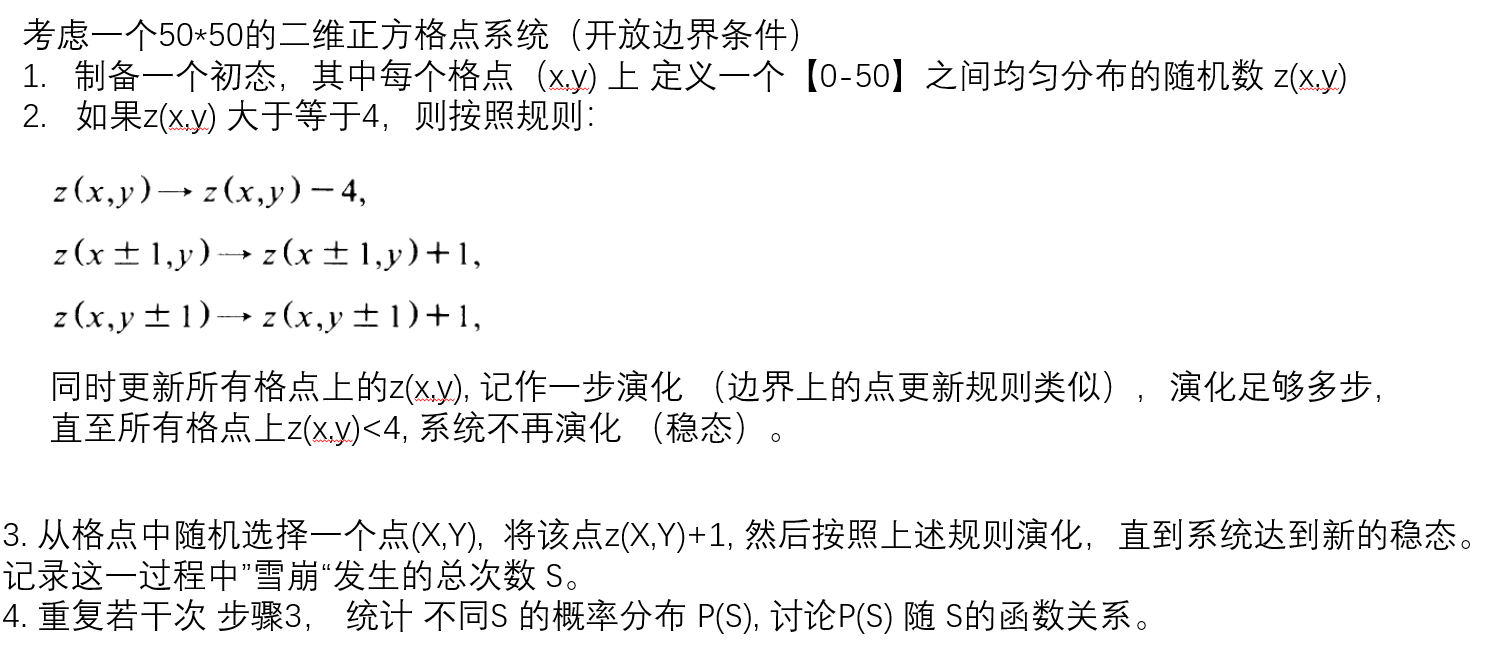
\includegraphics[width=1\textwidth,height=0.5\textwidth]{pictures/project.png}
		\caption{题目总览} \label{project}
	\end{figure}
  
  \newline

  由上可知,一个比较简单的思路就是统计每一轮中该矩阵的大于等于四的位点
  的坐标,然后在另一个空白矩阵的对应位点填上-4,以及上下左右位点的+1.
  而对于边界上的点,不妨填充一周的0,最后统计时只取中间的2-51行列即可。\newline

  观察到后面的对于雪崩次数$S$的需求,那么可以在每个循环额外增加一个
  对于雪崩次数的统计。\newline
\section{代码展示}

\subsubsection{前置函数编写}
以下为一步更新所用到的函数。\newline
~\\
\lstset{language=matlab}
\begin{lstlisting}
  function [z,S]=step(z,S)
%z为一次更新后的矩阵,S为雪崩发生次数
%扩展矩阵,进行补零
A=zeros(52,52);
A(2:51,2:51)=z;
%原始的处理矩阵
B=zeros(52,52);
for i=2:51
    for j=2:51
        if A(i,j)>=4
           B(i,j)=B(i,j)-4;
           B(i-1,j)=B(i-1,j)+1;
           B(i+1,j)=B(i+1,j)+1;
           B(i,j-1)=B(i,j-1)+1;
           B(i,j+1)=B(i,j+1)+1;
           S=S+1;
        end
    end
end
%同时演化一步
z=z+B(2:51,2:51);
end
\end{lstlisting}
以下为迭代函数,将一个矩阵更新至稳态为止。\newline

~\\
\lstset{language=matlab}
\begin{lstlisting}
  function [z,n,S]=update(z,S0)
  %输出稳态的z矩阵,n为本次更新次数,S为累计发生次数
  n=0;S=S0;
  while max(max(z))>=4
  [z,S]=step(z,S);
  n=n+1;
  end
  disp("本轮更新次数为"+n+",雪崩累计发生次数为"+S+",平均每轮雪崩"+S/n+"次")
  if max(max(z))<4
      disp("本轮未更新")
  end
  end  
\end{lstlisting}
以下为扰动函数,即随机选择一个位点使其值+1.\newline
~\\
\lstset{language=matlab}
\begin{lstlisting}
  function b=pert(z)
  %扰动函数,随机选择一个点使其值加一
  coord=randi(50,1,2);
  z(coord)=z(coord)+1;
  b=z;
  end 
\end{lstlisting}
\subsubsection{主体函数编写}
~\\
\lstset{language=matlab}
\begin{lstlisting}
  %%
%扰动后演化至稳定
%数据预备
clear;clc;
z=rand(50,50)*50;
S_series=zeros(1,10^6);%记录S频率用的列表
%先使矩阵处于稳态
z=update(z,0);
for l=1:length(S_series)
%先扰动,再使其演化为稳态
z=pert(z);
[z,~,S]=update(z,0);
S_series(l)=S;
end
histogram(S_series,10000)
xlabel("S雪崩次数")
ylabel("n(S)频率")
\end{lstlisting}
由此可以统计每一次随即位点+1之后发生雪崩的次数。
\section{结果分析与结论}
由于生成图像较为极端,所以下面将会按照总体和局部分别展示呈现的图像。
	\begin{figure}[!htbp]
		\centering
		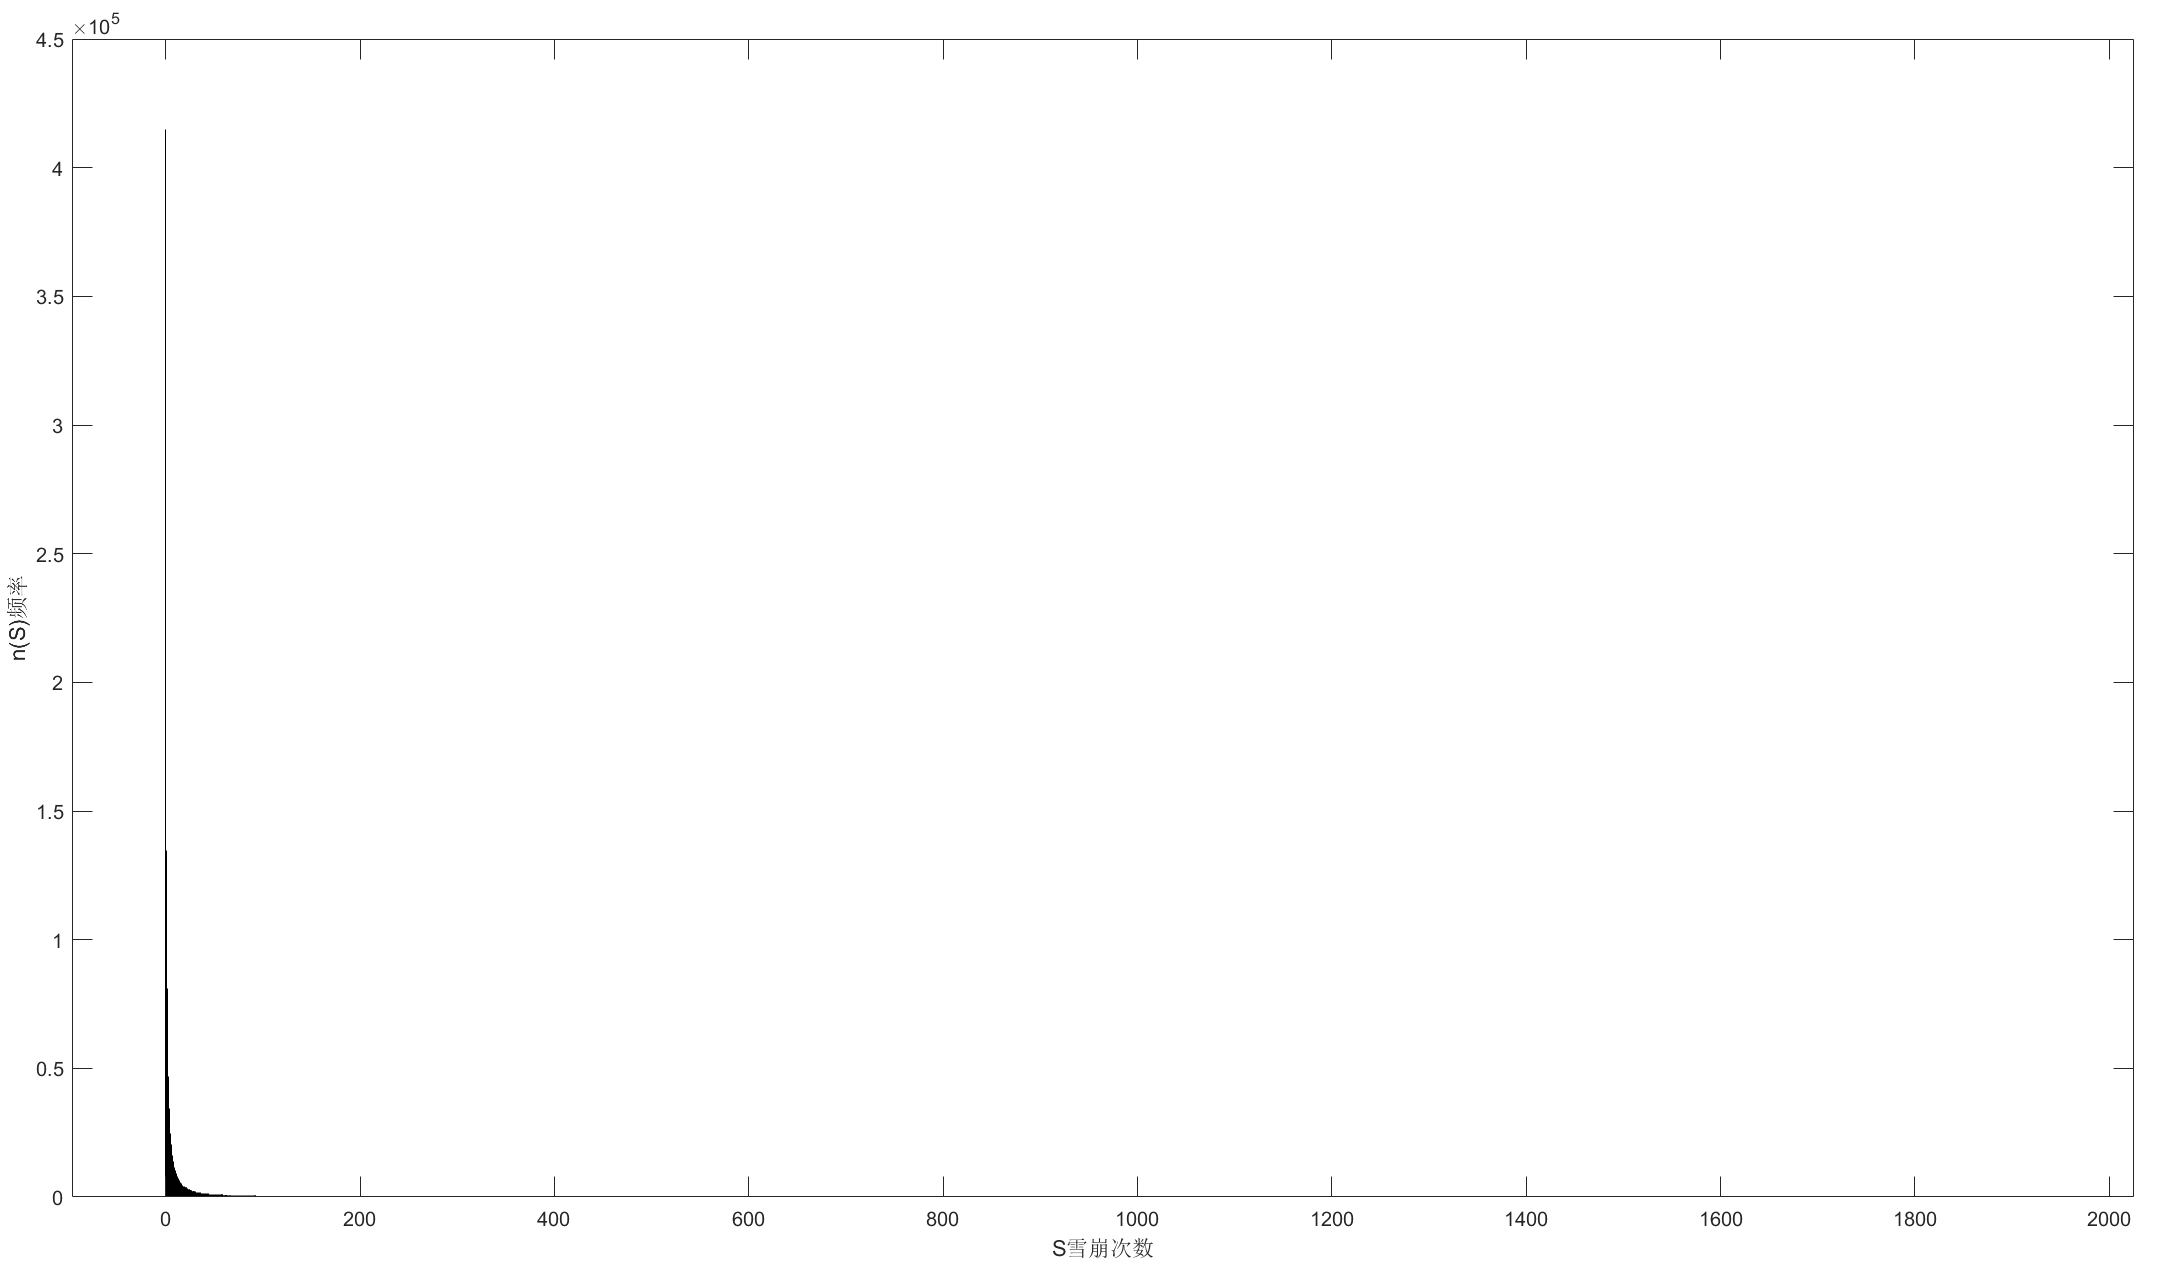
\includegraphics[width=1\textwidth,height=0.75\textwidth]{pictures/all.png}
		\caption{总览图} \label{all}
	\end{figure}
  \begin{figure}[!htbp]
		\centering
		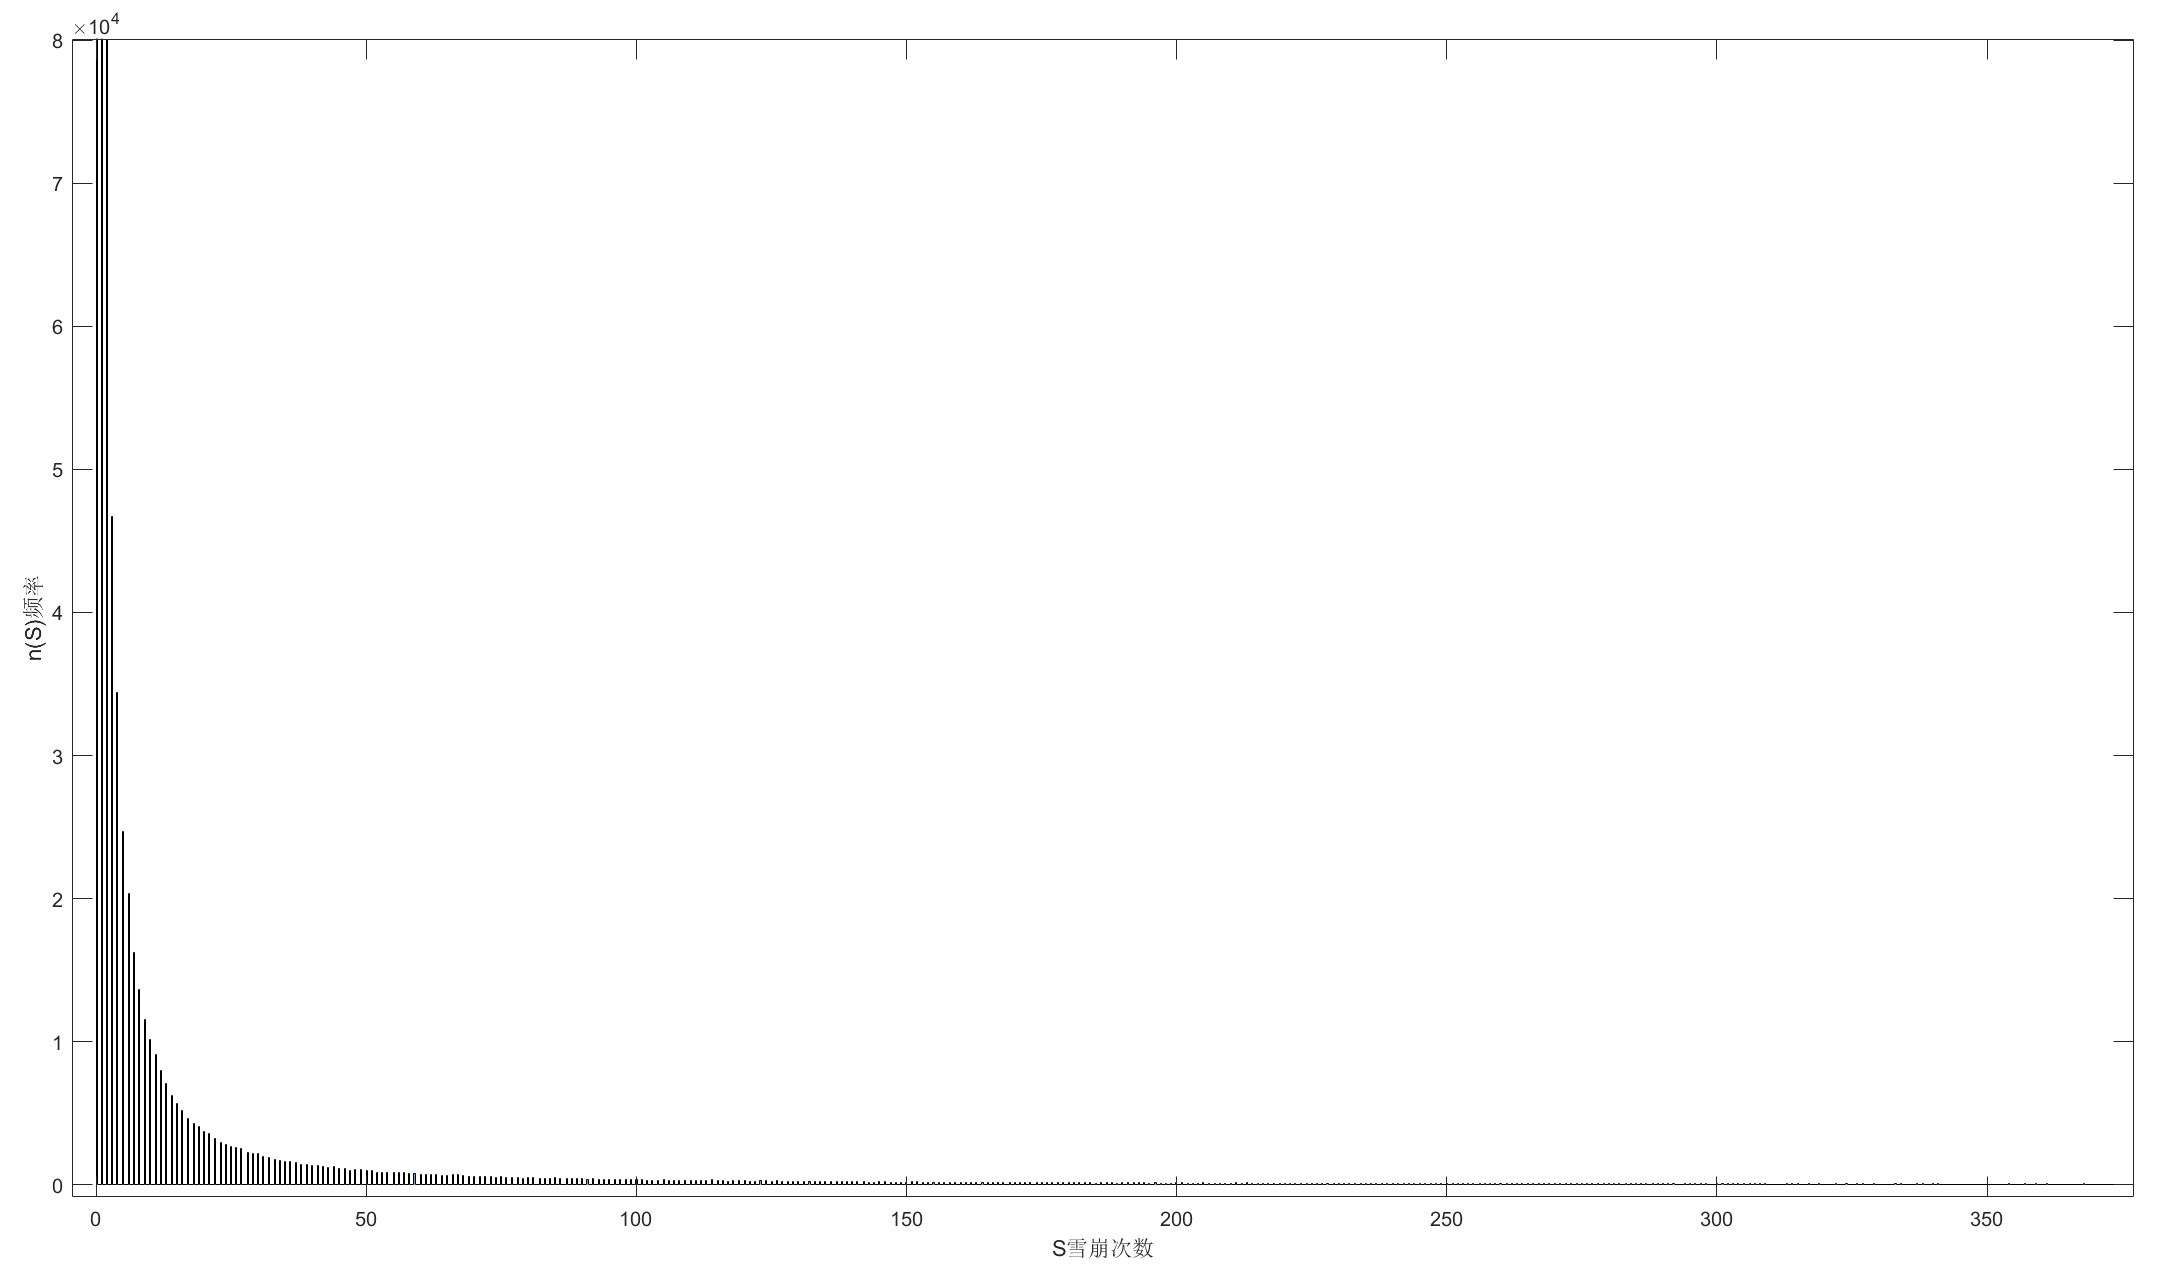
\includegraphics[width=1\textwidth,height=0.75\textwidth]{pictures/part.png}
		\caption{局部图} \label{part}
	\end{figure}
\newpage
由此可知,由于在绘制频率直方图时n(S)的区间取得非常小,所以可以近似看作为P(S)的相似图像,那么就可以看出,雪崩次数非常密集地聚集在了0~100次,从100次之后就开始变得逐渐稀薄,并且总体呈现出类似于反比例函数的图像。\newline
次数即使从0开始也是非常急剧的下降。
%以下为插入代码模板
%~\\
%\lstset{language=matlab}
%\begin{lstlisting}
%\end{lstlisting}


%%%以下为插入图片模板
%\quad \newline
%	\begin{figure}[!htbp]
%		\centering
%		\includegraphics[width=0.5\textwidth,height=0.375\textwidth]{pictures/minscale.png}
%		\caption{最小风向} \label{minsacle}
%	\end{figure}

%%%以下为插入图片模板
%\quad \newline
%	\begin{figure}[!htbp]
%		\centering
%		\includegraphics[width=0.5\textwidth,height=0.375\textwidth]{pictures/minscale.png}
%		\caption{最小风向} \label{minsacle}
%	\end{figure}

%    \begin{algorithm}
%		\caption{Title of the Algorithm}
%     	\begin{algorithmic}[1]
%			\REQUIRE some words.  % this command shows "Input"
%			\ENSURE ~\\           % this command shows "Initialized"
%			some text goes here ... \\
%			\WHILE {\emph{not converged}}
%			\STATE ... \\  % line number at left side
%			\ENDWHILE
%			\RETURN this is the lat part.  % this command shows "Output"
%		\end{algorithmic}
%	\end{algorithm}

\end{document}